% vim: set ft=tex tabstop=4 shiftwidth=4 noexpandtab:

% vim: set ft=tex tabstop=4 shiftwidth=4 noexpandtab:

% opening %{{{1

\documentclass[tikz, border=1mm]{standalone}

% packages and libraries %{{{1

% ---- not necessary since the documentclass[tikz ...] requires it automatically
% \usepackage{tikz}

\usetikzlibrary{calc,intersections,angles,quotes,shapes.geometric}

\usepackage{amsmath}

\usepackage{tkz-euclide}


% opening %{{{1

\begin{document}
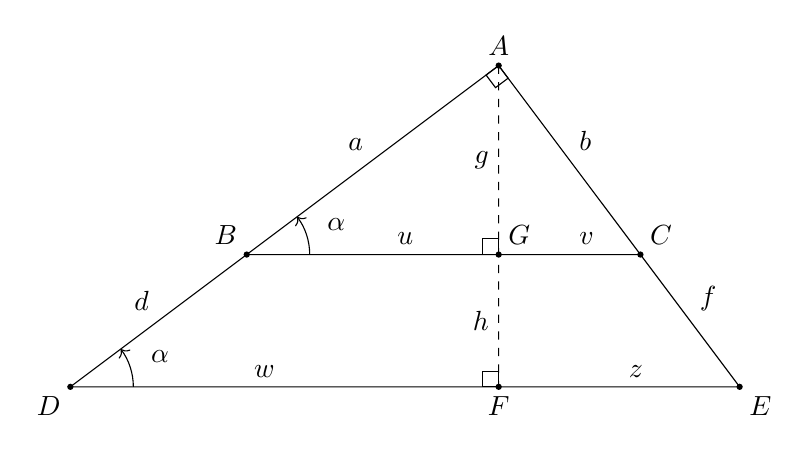
\begin{tikzpicture}[scale=1.0]

% parameters %{{{1

	\def\ratio{1.7}

	\tikzmath{
		\ang = atan2(-4, 3) - 90 ;
	}

% coordinates %{{{1

	\begin{scope}[rotate=\ang]
		\coordinate (A) at (0,0);
		\coordinate (B) at (4,0);
		\coordinate (C) at (0,3);
		\begin{scope}[scale=\ratio]
			\coordinate (D) at (4,0);
			\coordinate (E) at (0,3);
		\end{scope}
		\coordinate (F) at ($(D)!(A)!(E)$);
	\end{scope}

% intersections %{{{1

	\begin{pgfinterruptboundingbox}
		\path[name path=line1] (A) -- (F);
		\path[name path=line2] (B) -- (C);
		\path[name intersections={of=line1 and line2, by=G}];
	\end{pgfinterruptboundingbox}

% points, dots, vertices %{{{1

	\fill (A) circle (0.4mm);
	\fill (B) circle (0.4mm);
	\fill (C) circle (0.4mm);
	\fill (D) circle (0.4mm);
	\fill (E) circle (0.4mm);
	\fill (F) circle (0.4mm);
	\fill (G) circle (0.4mm);

% lines %{{{1

	\draw (A) -- (D) -- (E) -- cycle;
	\draw (B) -- (C);

	\draw[dashed] (A) -- (F);

% points, dots, vertices labels %{{{1

	\node[above] at (A) {$A$};
	\node[above left] at (B) {$B$};
	\node[above right] at (C) {$C$};
	\node[below left] at (D) {$D$};
	\node[below right] at (E) {$E$};
	\node[below] at (F) {$F$};
	\node[above right] at (G) {$G$};

	%\node[below left] at (A) {$A$};
	%\node[below] at (B) {$B$};
	%\node[left] at (C) {$C$};
	%\node[below right] at (D) {$D$};
	%\node[above] at (E) {$E$};
	%\node[above right] at (F) {$F$};
	%\node[above] at (G) {$G$};

% segments, sides, lines labels %{{{1

	\node[above left] at ($ (A)!0.5!(B) $) {$a$};
	\node[above right] at ($ (A)!0.5!(C) $) {$b$};

	\node[above left] at ($ (D)!0.5!(B) $) {$d$};
	\node[above right] at ($ (E)!0.5!(C) $) {$f$};

	\node[left] at ($ (A)!0.5!(G) $) {$g$};
	\node[left] at ($ (G)!0.5!(F) $) {$h$};

	\node[above left] at ($ (B)!0.7!(G) $) {$u$};
	\node[above right] at ($ (G)!0.5!(C) $) {$v$};

	\node[above left] at ($ (D)!0.5!(F) $) {$w$};
	\node[above right] at ($ (F)!0.5!(E) $) {$z$};

% angles labels %{{{1

	\pic[draw, ->, "$\alpha$", angle radius=0.8cm, angle eccentricity=1.5]
	{angle = C--B--A};

	\pic[draw, ->, "$\alpha$", angle radius=0.8cm, angle eccentricity=1.5]
	{angle = E--D--A};

% right angle marks %{{{2

	\tkzMarkRightAngle[size=0.2](B,A,C)
	\tkzMarkRightAngle[size=0.2](A,G,B)
	\tkzMarkRightAngle[size=0.2](A,F,D)

% closing %{{{1

\end{tikzpicture}
\end{document}
